% Options for packages loaded elsewhere
% Options for packages loaded elsewhere
\PassOptionsToPackage{unicode}{hyperref}
\PassOptionsToPackage{hyphens}{url}
%


\PassOptionsToPackage{table}{xcolor}

\documentclass[
  10pt,
  letterpaper,
]{article}
\usepackage{xcolor}
\usepackage[top=0.85in,left=2.75in,footskip=0.75in]{geometry}
\usepackage{amsmath,amssymb}
\setcounter{secnumdepth}{-\maxdimen} % remove section numbering
\usepackage{iftex}
\ifPDFTeX
  \usepackage[T1]{fontenc}
  \usepackage[utf8]{inputenc}
  \usepackage{textcomp} % provide euro and other symbols
\else % if luatex or xetex
  \usepackage{unicode-math} % this also loads fontspec
  \defaultfontfeatures{Scale=MatchLowercase}
  \defaultfontfeatures[\rmfamily]{Ligatures=TeX,Scale=1}
\fi
\usepackage{lmodern}
\ifPDFTeX\else
  % xetex/luatex font selection
\fi
% Use upquote if available, for straight quotes in verbatim environments
\IfFileExists{upquote.sty}{\usepackage{upquote}}{}
\IfFileExists{microtype.sty}{% use microtype if available
  \usepackage[]{microtype}
  \UseMicrotypeSet[protrusion]{basicmath} % disable protrusion for tt fonts
}{}
\makeatletter
\@ifundefined{KOMAClassName}{% if non-KOMA class
  \IfFileExists{parskip.sty}{%
    \usepackage{parskip}
  }{% else
    \setlength{\parindent}{0pt}
    \setlength{\parskip}{6pt plus 2pt minus 1pt}}
}{% if KOMA class
  \KOMAoptions{parskip=half}}
\makeatother


\usepackage{longtable,booktabs,array}
\newcounter{none} % for unnumbered tables
\usepackage{calc} % for calculating minipage widths
% Correct order of tables after \paragraph or \subparagraph
\usepackage{etoolbox}
\makeatletter
\patchcmd\longtable{\par}{\if@noskipsec\mbox{}\fi\par}{}{}
\makeatother
% Allow footnotes in longtable head/foot
\IfFileExists{footnotehyper.sty}{\usepackage{footnotehyper}}{\usepackage{footnote}}
\makesavenoteenv{longtable}
\usepackage{graphicx}
\makeatletter
\newsavebox\pandoc@box
\newcommand*\pandocbounded[1]{% scales image to fit in text height/width
  \sbox\pandoc@box{#1}%
  \Gscale@div\@tempa{\textheight}{\dimexpr\ht\pandoc@box+\dp\pandoc@box\relax}%
  \Gscale@div\@tempb{\linewidth}{\wd\pandoc@box}%
  \ifdim\@tempb\p@<\@tempa\p@\let\@tempa\@tempb\fi% select the smaller of both
  \ifdim\@tempa\p@<\p@\scalebox{\@tempa}{\usebox\pandoc@box}%
  \else\usebox{\pandoc@box}%
  \fi%
}
% Set default figure placement to htbp
\def\fps@figure{htbp}
\makeatother





\setlength{\emergencystretch}{3em} % prevent overfull lines

\providecommand{\tightlist}{%
  \setlength{\itemsep}{0pt}\setlength{\parskip}{0pt}}



 
\usepackage[numbers,square,comma]{natbib}
\bibliographystyle{plos2015}


% Use adjustwidth environment to exceed column width (see example table in text)
\usepackage{changepage}

% marvosym package for additional characters
\usepackage{marvosym}

% cite package, to clean up citations in the main text. Do not remove.
% Using natbib instead
% \usepackage{cite}

% Use nameref to cite supporting information files (see Supporting Information section for more info)
\usepackage{nameref,hyperref}

% line numbers
\usepackage[right]{lineno}

% ligatures disabled
\usepackage{microtype}
\DisableLigatures[f]{encoding = *, family = * }

% create "+" rule type for thick vertical lines
\newcolumntype{+}{!{\vrule width 2pt}}

% create \thickcline for thick horizontal lines of variable length
\newlength\savedwidth
\newcommand\thickcline[1]{%
  \noalign{\global\savedwidth\arrayrulewidth\global\arrayrulewidth 2pt}%
  \cline{#1}%
  \noalign{\vskip\arrayrulewidth}%
  \noalign{\global\arrayrulewidth\savedwidth}%
}

% \thickhline command for thick horizontal lines that span the table
\newcommand\thickhline{\noalign{\global\savedwidth\arrayrulewidth\global\arrayrulewidth 2pt}%
\hline
\noalign{\global\arrayrulewidth\savedwidth}}

% Text layout
\raggedright
\setlength{\parindent}{0.5cm}
\textwidth 5.25in 
\textheight 8.75in

% Bold the 'Figure #' in the caption and separate it from the title/caption with a period
% Captions will be left justified
\usepackage[aboveskip=1pt,labelfont=bf,labelsep=period,justification=raggedright,singlelinecheck=off]{caption}
\renewcommand{\figurename}{Fig}

% Remove brackets from numbering in List of References
\makeatletter
\renewcommand{\@biblabel}[1]{\quad#1.}
\makeatother

% Header and Footer with logo
\usepackage{lastpage,fancyhdr}
\usepackage{epstopdf}
%\pagestyle{myheadings}
\pagestyle{fancy}
\fancyhf{}
%\setlength{\headheight}{27.023pt}
%\lhead{\includegraphics[width=2.0in]{PLOS-submission.eps}}
\rfoot{\thepage/\pageref{LastPage}}
\renewcommand{\headrulewidth}{0pt}
\renewcommand{\footrule}{\hrule height 2pt \vspace{2mm}}
\fancyheadoffset[L]{2.25in}
\fancyfootoffset[L]{2.25in}
\lfoot{\today}
\makeatletter
\@ifpackageloaded{float}{}{\usepackage{float}}
\floatstyle{plain}
\@ifundefined{c@chapter}{\newfloat{suppfig}{h}{losuppfig}}{\newfloat{suppfig}{h}{losuppfig}[chapter]}
\floatname{suppfig}{Figure S}
\newcommand*\quartosuppfigref[1]{Figure \hyperref[#1]{S\ref{#1}}}
\@ifpackageloaded{caption}{}{\usepackage{caption}}
\DeclareCaptionLabelFormat{quartosuppfigreflabelformat}{#1#2}
\captionsetup[suppfig]{labelformat=quartosuppfigreflabelformat}
\newcommand*\listofsuppfigs{\listof{suppfig}{List of Supplementary Figures}}
\makeatother
\makeatletter
\@ifpackageloaded{float}{}{\usepackage{float}}
\floatstyle{plain}
\@ifundefined{c@chapter}{\newfloat{supptbl}{h}{losupptbl}}{\newfloat{supptbl}{h}{losupptbl}[chapter]}
\floatname{supptbl}{Table S}
\floatstyle{plaintop}
\restylefloat{supptbl}
\newcommand*\quartosupptblref[1]{Table \hyperref[#1]{S\ref{#1}}}
\@ifpackageloaded{caption}{}{\usepackage{caption}}
\DeclareCaptionLabelFormat{quartosupptblreflabelformat}{#1#2}
\captionsetup[supptbl]{labelformat=quartosupptblreflabelformat}
\newcommand*\listofsupptbls{\listof{supptbl}{List of Supplementary Tables}}
\makeatother
\makeatletter
\@ifpackageloaded{caption}{}{\usepackage{caption}}
\AtBeginDocument{%
\ifdefined\contentsname
  \renewcommand*\contentsname{Table of contents}
\else
  \newcommand\contentsname{Table of contents}
\fi
\ifdefined\listfigurename
  \renewcommand*\listfigurename{List of Figures}
\else
  \newcommand\listfigurename{List of Figures}
\fi
\ifdefined\listtablename
  \renewcommand*\listtablename{List of Tables}
\else
  \newcommand\listtablename{List of Tables}
\fi
\ifdefined\figurename
  \renewcommand*\figurename{Figure}
\else
  \newcommand\figurename{Figure}
\fi
\ifdefined\tablename
  \renewcommand*\tablename{Table}
\else
  \newcommand\tablename{Table}
\fi
}
\@ifpackageloaded{float}{}{\usepackage{float}}
\floatstyle{ruled}
\@ifundefined{c@chapter}{\newfloat{codelisting}{h}{lop}}{\newfloat{codelisting}{h}{lop}[chapter]}
\floatname{codelisting}{Listing}
\newcommand*\listoflistings{\listof{codelisting}{List of Listings}}
\makeatother
\makeatletter
\makeatother
\makeatletter
\@ifpackageloaded{caption}{}{\usepackage{caption}}
\@ifpackageloaded{subcaption}{}{\usepackage{subcaption}}
\makeatother
\usepackage{bookmark}
\IfFileExists{xurl.sty}{\usepackage{xurl}}{} % add URL line breaks if available
\urlstyle{same}
\hypersetup{
  pdftitle={Mechanical power output during stretch--shortening cycles of rat medial gastrocnemius muscle: influence of various muscle length trajectories},
  pdfauthor={Edwin D.H.M. Reuvers; Huub Maas; Wendy Noort; Maarten F. Bobbert; Dinant A. Kistemaker},
  hidelinks,
  pdfcreator={LaTeX via pandoc}}




\begin{document}
\vspace*{0.2in}

% Title must be 250 characters or less.
\begin{flushleft}
{\Large
\textbf\newline{Mechanical power output during stretch--shortening
cycles of rat medial gastrocnemius muscle: influence of various muscle
length
trajectories} % Please use "sentence case" for title and headings (capitalize only the first word in a title (or heading), the first word in a subtitle (or subheading), and any proper nouns).
}
\newline
\\
% Insert author names, affiliations and corresponding author email (do not include titles, positions, or degrees).
Edwin D.H.M. Reuvers\textsuperscript{1*}, Huub
Maas\textsuperscript{1}, Wendy Noort\textsuperscript{1}, Maarten F.
Bobbert\textsuperscript{1}, Dinant A. Kistemaker\textsuperscript{1}
\\
\bigskip
\textbf{1} Department of Human Movement Sciences, Faculty of Behavioural
and Movement Sciences, Vrije Universiteit Amsterdam, Amsterdam Movement
Sciences, The Netherlands, Amsterdam, 1081 BT, The Netherlands, 
\bigskip

% Insert additional author notes using the symbols described below. Insert symbol callouts after author names as necessary.
% 
% Remove or comment out the author notes below if they aren't used.
%
% Primary Equal Contribution Note

% Additional Equal Contribution Note
% Also use this double-dagger symbol for special authorship notes, such as senior authorship.
%\ddag These authors also contributed equally to this work.

% Current address notes

% Deceased author note

% Group/Consortium Author Note

% Use the asterisk to denote corresponding authorship and provide email address in note below.
* edwin.reuvers.academia@pm.me

\end{flushleft}

\section*{Abstract}
The average mechanical power output (AMPO) during a stretch--shortening
cycle produced by a muscle depends on muscle length and stimulation over
time. While the effects of cycle frequency and muscle length excursion
on AMPO are well-known, several questions remain about the effects of
muscle length and stimulation over time on the maximally attainable
AMPO. For example, which precise muscle length and stimulation over time
yield maximal AMPO? \emph{In situ} experiments are inherently limited to
a finite set of muscle length and stimulation over time. To overcome
this limitation, we combined \emph{in situ} experiments on rat \emph{m.
gastrocnemius medialis} with Hill-type muscle modelling. We first
performed dedicated trials to estimate the muscle-tendon-complex (MTC)
properties of each rat. Subsequently, we performed various
stretch--shortening cycles with substantial differences in cycle
frequency, shortening-to-lengthening time ratio and MTC length
excursion. Model-predicted AMPO correlated nearly perfectly with
experimentally measured AMPO (r² \textgreater{} 0.98). This justified
further exploration using the Hill-type MTC model. Using the Hill-type
MTC model, we predicted that AMPO peaks at a cycle frequency of 3.5 Hz,
with a shortening-to-lengthening time ratio of 6:1 and an MTC length
excursion of 8 mm. Notably, cycle frequency and MTC length excursion
showed a strong interaction: increasing one necessitated a decrease in
the other to maximise AMPO. By contrast, the optimal
shortening-to-lengthening time ratio remained remarkably constant across
all tested combinations of cycle frequency and MTC length excursion.
This shows that muscles should spend substantially more time shortening
than lengthening to maximise AMPO.


\newgeometry{top=0.85in,left=1in,right=1in,footskip=0.75in}
\linenumbers

\nolinenumbers

\subsection*{Author summary}\label{author-summary}
\addcontentsline{toc}{subsection}{Author summary}

The average mechanical power output (AMPO) during cyclic contractions,
in which a muscle shortens and lengthens, is a key determinant of
performance in tasks like sprint cycling and rowing. Apart from
stimulation muscle AMPO depends on three key factors: cycle frequency
(the number of shortening--lengthening cycles per second), length
excursion (the change in muscle length during each cycle), and the
relative duration of shortening and lengthening. To study the dependency
of AMPO on these key factors, we combined experiments on rat calf muscle
with a mathematical muscle model incorporating key physiological
properties. The model accurately reproduced the experimental results,
which allowed us to explore a much wider range of the three factors than
would be possible using experiments alone. Cycle frequency and length
excursion interacted strongly, such that increasing one required
decreasing the other to maximise AMPO. By contrast, the optimal relative
duration of shortening and lengthening was consistent across all tested
cycle frequencies and length excursions: AMPO was maximised when muscles
spent about 85\% of each cycle shortening. These findings improve our
understanding of muscle function and may help explain animal behaviour
as well as inform sports equipment design to enhance performance.

\linenumbers

\subsection{Introduction}\label{introduction}

In motor activities such as cycling, rowing, and speed skating, muscles
periodically shorten and lengthen, a pattern commonly referred to as the
stretch--shortening cycle (SSC). When muscles produce force while
shortening, they deliver positive mechanical power, and when they
produce force while lengthening, they deliver negative mechanical power.
During motor activities, part of the mechanical energy delivered by the
muscles is dissipated to the environment, and this energy loss generally
increases with movement speed. Consequently, performance critically
depends on the average mechanical power output (AMPO) that muscles can
produce over these SSCs. This raises several fundamental questions: how
does muscle length over time influence the maximally attainable AMPO?
More specifically, what are the effects of cycle frequency and muscle
length excursion? Which fraction of the cycle should be spent
shortening? And (how) do these factors interact? Surprisingly, despite
the importance of AMPO for movement performance, many of these questions
have not yet been answered.

To study the mechanical output during a stretch--shortening cycle (SSC),
researchers use an experimental setup in which a motor imposes cyclical
length changes on either isolated muscle fibres or the entire
muscle--tendon complex (MTC). While the approach is the same at both
levels, this paper focuses on SSCs at the MTC level. During each SSC,
the MTC first undergoes lengthening and then shortens back to its
initial length. Muscle stimulation is applied during part of the SSC,
while MTC force is measured. When MTC force is plotted against MTC
length (change), the area enclosed by the resulting loop represents the
net mechanical work produced during a full cycle. This net mechanical
work is the sum of the positive mechanical work during MTC shortening
(Fig~\ref{fig-i-workloop}A) and the negative mechanical work during MTC
lengthening (Fig~\ref{fig-i-workloop}B). This method has been coined the
`work loop technique' \citep{josephson_mechanical_1985}. The average
mechanical power output (AMPO) for each cycle can then be calculated by
dividing the net mechanical work per cycle by the duration of the cycle.
As such, the work loop technique provides a powerful tool to study the
effect of MTC length and stimulation over time on the maximally
attainable AMPO of muscles.

\begin{figure}[h]

\centering{

\pandocbounded{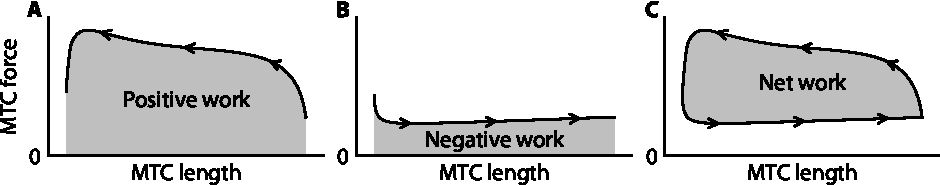
\includegraphics[keepaspectratio]{../figures/i_workloop.pdf}}

}

\caption{\label{fig-i-workloop}\textbf{An example of a work loop.} In a
work loop, MTC force is plotted against MTC length (change). The area
enclosed by the work loop represents the net mechanical work produced
during a full cycle (C), which is the sum of the positive mechanical
work during MTC shortening (A) and the negative mechanical work during
MTC lengthening (B). The arrows indicate the direction of the work loop
over time.}

\end{figure}%

The work loop technique has been extensively employed to examine how MTC
(or muscle fibre) length and muscle stimulation over time affect the
mechanical behaviour of muscles. In most experiments, SSCs have been
studied using sinusoidal length changes
\citep[e.g.][]{josephson_mechanical_1985}. These SSCs are typically
parametrised in terms of cycle frequency and MTC/muscle fibre length
excursion, with length changes centred around the length yielding
maximal isometric force. Furthermore, muscle stimulation is typically
parametrised in terms of stimulation onset time and stimulation duration
(i.e.~`duty cycle'). Since muscle stimulation substantially affects the
mechanical behaviour of muscles
\citep[e.g.][]{curtin_remarkable_2018, sawicki_timing_2015, stevens_pattern_1996},
stimulation onset time and duration are typically optimised to maximise
mechanical work per cycle. This allows isolation of the effects of cycle
frequency and MTC/muscle fibre length excursion, and their interaction.
Such an approach has been used in experiments to systematically
investigate both the individual effects of cycle frequency and
MTC/muscle fibre length excursion and their interaction on AMPO. For
example, results from such experiments have demonstrated a substantial
interaction between cycle frequency and MTC/muscle fibre length
excursion, whereby maximising AMPO typically requires larger length
excursions at lower frequencies and smaller length excursions at higher
frequencies
\citep[e.g.][]{altringham_modelling_1990, james_mechanical_1995, caiozzo_determinants_1997}.
Although sinusoidal SSCs have experimentally provided valuable insights,
they inherently impose equal shortening and lengthening durations,
leaving unexplored how unequal shortening and lengthening durations
affect AMPO.

Askew \& Marsh {\citep{askew_effects_1997, askew_optimal_1998}}
performed ground-breaking experiments on the effect of unequal
shortening and lengthening durations on the maximally attainable AMPO
--- remaining, to our knowledge, the only researchers to have done so.
In their studies, mouse \emph{m. soleus} and \emph{m. extensor digitorum
longus} were connected at the distal part of the muscle belly to a
servomotor for precise control of the imposed SSCs. The SSCs used by
Askew \& Marsh were parameterised using three variables (see
Fig~\ref{fig-i-ssc-parameterisation}): cycle frequency, FTS (fraction of
the cycle time spent shortening), and muscle fibre length excursion
(i.e.~maximum minus minimum fibre length), with near-constant shortening
and lengthening velocities. Askew \& Marsh
{\citep{askew_effects_1997, askew_optimal_1998}} examined three distinct
FTS values --- 0.25, 0.50, and 0.75 --- and heuristically optimised
muscle fibre length excursion, muscle stimulation onset time and muscle
stimulation duration to achieve the highest AMPO at different
combinations of cycle frequency and FTS. Their findings indicated that
AMPO was highest for FTS = 0.75, followed by FTS = 0.50, and lowest for
FTS = 0.25 at each cycle frequency at the optimal muscle fibre length
excursion and muscle stimulation.

\begin{figure}[h]

\centering{

\pandocbounded{
\includegraphics[keepaspectratio]{../figures/i_ssc_parameterisation.pdf}}

}

\caption{\label{fig-i-ssc-parameterisation}\textbf{Representation of the
parameterisation of stretch--shortening cycles.} \(T_{short}\) and
\(T_{length}\) denote the shortening and lengthening durations,
respectively, of either the muscle-tendon-complex (MTC) or the muscle
fibres. FTS denotes the fraction of the cycle time spent shortening. In
the example shown, the MTC/muscle fibres shorten 65\% of the cycle
duration (i.e.~FTS = 0.65).}

\end{figure}%

While Askew \& Marsh's experimental studies provided valuable insights,
several questions remain regarding the effect of SSC parameters on the
maximally attainable AMPO. First, Askew \& Marsh
{\citep{askew_effects_1997, askew_optimal_1998}} optimised muscle fibre
length excursion for each cycle frequency at only three distinct FTS
values. Therefore, it remains unclear how muscle fibre length excursion
affects the maximally attainable AMPO at different FTS values. More
generally, it remains unclear how sensitive the maximally attainable
AMPO is to variations in SSC parameters. For instance, does AMPO
substantially decrease with suboptimal SSC parameters, or is there a
wide range of SSC parameter combinations that yield near-maximal AMPO?
Second, because Askew \& Marsh
{\citep{askew_effects_1997, askew_optimal_1998}} only used three
distinct FTS values, it remains unclear how cycle frequency and muscle
fibre length excursion affect the optimum value of FTS. More generally,
it remains unclear how the optimum SSC parameters depend on each other.
Third, Askew \& Marsh {\citep{askew_effects_1997, askew_optimal_1998}}
imposed near-constant muscle fibre shortening and lengthening
velocities. Consequently, it remains unclear how much more AMPO the
muscle could produce if the muscle fibre length over time would be
optimal for AMPO. For this, the optimal muscle fibre length and
stimulation over time should be identified in a parameter-free manner.

While it is obvious that muscle fibres should maximise positive
mechanical work and minimise negative mechanical work in order to
maximise AMPO, it is far from trivial what SSC and muscle stimulation
over time yield maximal AMPO. To minimise negative mechanical work,
stimulation should cease well before lengthening begins (because of
deactivation time delays) and muscle fibres should ideally lengthen at
very low velocities (as muscle fibre force increases with increasing
lengthening velocity). However, such strategies are suboptimal for AMPO:
the time spent lengthening cannot be used to produce positive mechanical
work, and early deactivation reduces the positive mechanical work during
shortening. One might argue that muscle fibres should shorten at a
velocity that maximises the instantaneous mechanical power output to
maximise positive mechanical work. However, muscle fibre force also
depends on muscle fibre length, with muscle fibre force decreasing at
both shorter and longer lengths than optimum length. Therefore, to
maximise AMPO, it may be beneficial for muscle fibres to contract at a
lower velocity than the velocity which maximises instantaneous
mechanical power output. Doing so limits the negative effects of
operating at suboptimal muscle fibre lengths. This raises several open
questions: What shortening velocity maximises AMPO? Over what length
range should muscle fibres operate? And how much time should be spent on
shortening (to maximise positive mechanical work) versus lengthening (to
minimise negative mechanical work) in order to maximise AMPO?

Obviously, it is hard to experimentally find the optimal combination of
cycle frequency, FTS, MTC length excursion and muscle stimulation for
maximal AMPO. If one would change MTC length excursion, how should the
other SSC parameters and muscle stimulation be changed to maximise AMPO?
Or, taking it one step further: How should we find the MTC length and
stimulation over time that maximises AMPO when the muscle length over
time is entirely free to take any form? For this reason, we propose to
complement \emph{in situ} experiments with simulations and optimisations
using a Hill-type MTC model to study the effects of MTC length and
muscle stimulation over time on the maximally attainable AMPO. If the
MTC model yields accurate predictions of the influence of SSC parameters
and muscle stimulation over time on the maximally attainable AMPO, it
would allow us to answer a plethora of questions regarding the maximally
attainable AMPO of various SSCs. For instance, we could investigate how
the optimum SSC parameters depend on each other, and how sensitive the
maximally attainable AMPO is to variations in SSC parameters.
Furthermore, using an accurate model, we could optimise MTC length over
time for maximal AMPO and quantify how much more AMPO could be produced
compared to sinusoidal SSCs or the near-constant velocity SSCs used by
Askew \& Marsh.

In this study, we aimed to explore the influence of SSC parameters ---
cycle frequency, FTS and MTC length excursion --- on the maximally
attainable AMPO of a single isolated MTC. Thus, we considered the
maximally attainable AMPO for each combination of SSC parameters. To
determine this, muscle stimulation was optimised for every SSC. As
discussed earlier, only a limited set of SSCs can be investigated
experimentally, so this raises the question: Which SSCs should be
selected? To make an informed selection of SSCs to be tested
experimentally, we first used a Hill-type MTC model --- with parameter
values obtained from literature --- to simulate a broad range of SSCs.
Based on these simulation results, we selected a smaller, representative
and informative set of SSCs that captured the most prominent effects,
providing a focused basis for evaluating model predictions. This set of
SSCs was then tested in an \emph{in situ} experiment on rat \emph{m.
gastrocnemius medialis}. In this experiment, we also performed dedicated
trials to estimate the MTC properties of each specimen individually.
This allowed us to compare the experimental results with model-based
predictions, which showed a nearly perfect correlation between measured
and model-predicted AMPO (r\textsuperscript{2} \textgreater{} 0.98).
This strong correspondence then justified the use of the Hill-type MTC
model to (finally) explore how SSC parameters --- cycle frequency, FTS
and MTC length excursion --- affect the maximally attainable AMPO and to
identify the fully unconstrained optimal MTC length over time for
maximal AMPO.

\subsection{Methods}\label{methods}

We combined \emph{in situ} experiments with simulations and
optimisations using a Hill-type MTC model to investigate the influence
of SSC parameters --- cycle frequency, FTS, and MTC length excursion ---
on the maximally attainable AMPO of rat \emph{m. gastrocnemius medialis}
(GM). We first used a Hill-type MTC model with parameter values from
literature to simulate a broad range of SSCs. Based on these simulation
results, we selected a representative and informative subset for an
\emph{in situ} experiment, in which MTC length and stimulation over time
were under full control. In this experiment, we also performed dedicated
trials to estimate the MTC properties of each specimen individually.
Model-based predictions were then evaluated against the experimental
data. The strong correspondence (r\textsuperscript{2} \textgreater{}
0.98) justified the use of the Hill-type MTC model to explore the
influence of SSC parameters on the maximally attainable AMPO across a
broad SSC parameter space. First, we derived predictions for SSCs with
constant MTC shortening and lengthening velocity. Second, we identified
the optimal SSC without any constraints on MTC length over time to
investigate how much more AMPO the muscle could produce if the muscle
were allowed to shorten-and-lengthen optimally.

\subsubsection{\texorpdfstring{\emph{In situ}
experiment}{In situ experiment}}\label{in-situ-experiment}

\paragraph{Animals and ethics}\label{animals-and-ethics}

All surgical and experimental procedures conducted in this study were
approved by the Committee on the Ethics of Animal Experimentation at the
Vrije Universiteit (Permit Number: FBW-AVD11200202114471) and adhered to
Dutch law concerning the guidelines and regulations of animal welfare
and experimentation. Data was obtained from three male Wistar rats (body
mass 365, 410 and 407 gram, respectively). The rats were anaesthetised
by intraperitoneally injecting a urethane solution (12.5\% urethane) at
a dosage of 1.2 mL/100 g body mass. Additional doses of urethane (0.2
mL/g body mass) were administered throughout the experiment as needed to
maintain deep anaesthesia Heart rate, body temperature and withdrawal
reflexes to a pain stimulus were monitored every 10 minutes. To prevent
dehydration, subcutaneous injections of 1 mL NaCl solution (0.9\%) were
administered every 1--2 hours. After completion of the experiment, we
euthanised the rats by intracardially injecting pentobarbital sodium
(Euthasol 20\%) followed by a double-sided pneumothorax.

\paragraph{Surgical procedure}\label{surgical-procedure}

The hindlimb of the rat was shaved, and the skin was cut and partially
removed. Next, \emph{m. biceps femoris} was removed to expose the femur.
To minimise mechanical effects of surrounding muscles on GM --- in
particular myofascial force transmission --- the following steps were
taken \citep[see][]{rijkelijkhuizen_extramuscular_2005}: 1) GM was
exposed as much as possible from its surrounding tissue. 2) The tendons
of \emph{m. plantaris}, \emph{m. gastrocnemius lateralis} and \emph{m.
soleus} were cut at their distal ends. 3) The medial and lateral parts
of \emph{m. gastrocnemius} were carefully separated. \emph{N. peroneus},
\emph{n.~suralis}, and the branch of the \emph{n.~tibialis} innervating
\emph{m. gastrocnemius lateralis} and \emph{m. soleus} were then cut to
further reduce the influence of surrounding tissue on GM. Subsequently,
the tissue around the calcaneal tendon was removed such that only a
small part of the calcaneus was left. Lastly, a cuff-electrode was
placed on \emph{n.~ischiadicus}. The part of \emph{n.~ischiadicus}
proximal to the cuff-electrode was then crushed to prevent muscle
excitation via spinal reflexes.

\paragraph{Experimental setup}\label{experimental-setup}

The rats were placed on an electrical heating pad to maintain body
temperature at 37 \(^{\circ}\)C. The laboratory temperature was kept
constant at 20 \(^{\circ}\)C, with a local humidity around the muscle
tissue of about 80\%. A servomotor (Aurora 309C, Aurora Scientific,
Aurora, Canada) was used to impose MTC length changes and to measure GM
force. Before the experiment, we calibrated the position sensor of the
servomotor using a dial gauge (2046S, Mitutoyo Nederland BV, Veenendaal,
the Netherlands) and calibrated the force sensor using various
calibration masses. To relate servomotor position (changes) to MTC
length, we measured MTC length at one position with a caliper at the end
of the experiment. A direct current stimulator was used to stimulate
\emph{n.~ischiadicus} with a pulse width of 100 \(\mu\)s and at a
frequency of 100 Hz during all experiments, while the (supramaximal)
current was chosen for every rat individually. Before the series of
experiments, we ensured that the position, force, and stimulation
signals were synchronised in time by applying a physical stimulus that
produced a detectable response across all channels. All data were
collected at a sample rate of 2000 Hz.

The femur was fixed with a metal clamp and the foot with a plastic
plate, such that the hindlimb was rigidly secured to the setup. The
distal end of the calcaneal bone was tightly attached to a steel rod
with 100\% polyester yarn at the leftover part of the calcaneus. The
other end of the steel rod was then attached with Kevlar thread to the
motor. A similar procedure was applied to \emph{m. gastrocnemius
lateralis} (GL) and \emph{m. plantaris} (PL). The distal tendon of GL
and PL (GL+PL) was then connected to a second motor to monitor their
combined force throughout the experiment in order to verify the absence
of mechanical interaction with GM. Care was taken to ensure that the
direction of GM force reflected \emph{in vivo} conditions. Lastly, we
connected the cuff-electrode to the direct current stimulator (DS2A,
Digitimer, Welwyn Garden City, United Kingdom). This setup allowed us to
have full control over MTC length and stimulation while measuring GM
force (see Fig~\ref{fig-m-setup}).

\begin{figure}[h]

\centering{

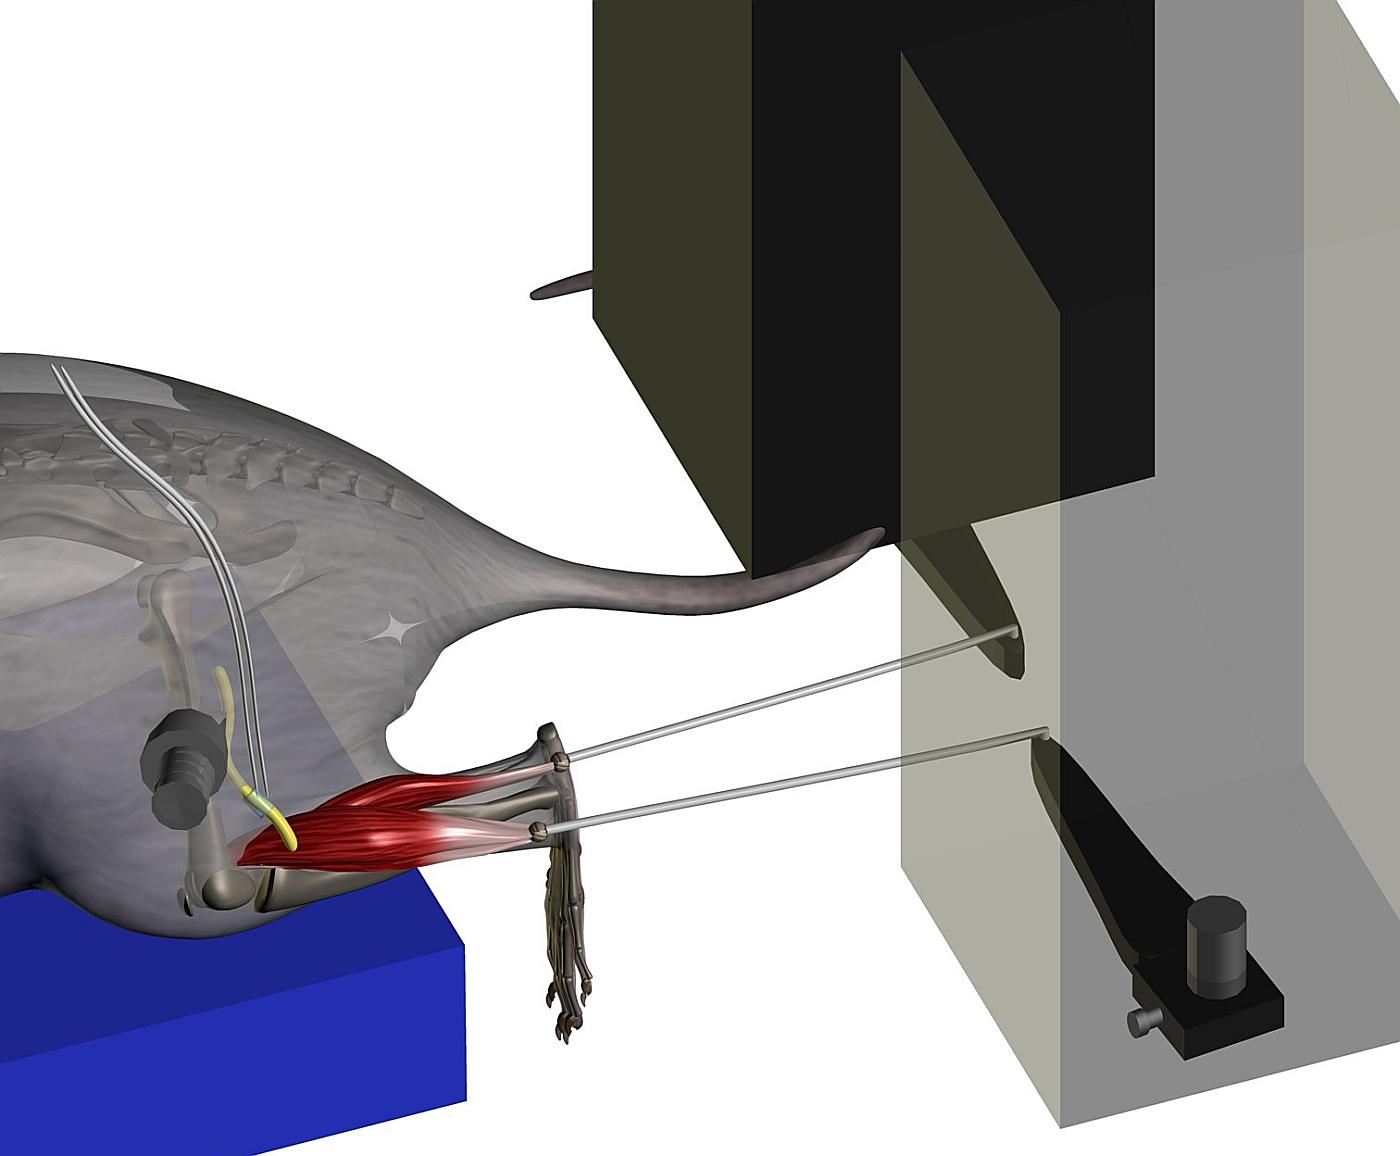
\includegraphics[width=7.96cm,height=\textheight,keepaspectratio]{../figures/m_setup.png}

}

\caption{\label{fig-m-setup}\textbf{Representation of the experimental
setup that provided full control of MTC length and stimulation while
measuring \emph{m. gastrocnemius medialis} (GM) force.} GM was carefully
exposed from its surrounding tissue and positioned in the setup such
that GM pulled in its natural direction, while the femur and foot were
securely fixated. The distal end of the calcaneal tendon was connected
to a motor via a steel rod. The distal tendon of \emph{m. gastrocnemius
lateralis} and \emph{m. plantaris} was connected to a second motor. A
cuff-electrode was placed on \emph{n.~ischiadicus}. \emph{N. peroneus},
\emph{n.~suralis} and the branch of \emph{n.~ischiadicus} innervating
\emph{m. gastrocnemius lateralis} and \emph{m. soleus} were cut such
that only GM was innervated.}

\end{figure}%

\paragraph{General procedures}\label{general-procedures}

After securing the rat in the experimental setup, we conducted a series
of tetanic contractions for several purposes. First, we performed
isometric contractions to ensure that GM pulled in its natural
direction. These isometric contractions were also used to determine the
supramaximal stimulation current for GM. The stimulation current was
gradually increased until GM force plateaued. The current at which no
further increase in GM force was observed was then used consistently
throughout the experiment. Additionally, the isometric contractions
served as a check to confirm that the surgery was successful,
particularly ensuring that no GL+PL force was transmitted to the distal
GL+PL tendon, and thus that no myofascial force transmission occurred
\citep{finni_force_2023}. Subsequently, we performed two to three
quick-release, step-ramp and isometric experiments along with two to
three SSCs. This approach was based on results from pilot experiments,
which indicated that imposing these contractions prior to the start of
the experiment resulted in more stable GM force throughout the entire
experiment.

Following the preparatory procedures, we commenced the main experiment.
The main experiment consisted of two parts. In the first part, we
performed quick-release, step-ramp and isometric experiments to estimate
the MTC properties of each rat. In the second part, we performed various
SSCs. To assess if GM was fatigued, two quick-release and two step-ramp
experiments were repeated halfway through the second part of the
experiment and again at the end of the entire experiment. Additionally,
isometric experiments were performed after every six series of SSCs
during the second part of the experiment, using a fixed MTC length 2-4
mm below MTC optimum length. Between contractions, GM was returned to
slack length, followed by a two-minute rest period. During these rest
periods, GM was irrigated with saline to keep the muscle tissue moist.
To reduce potentiation effects, two twitches were applied 1.5 seconds
before each contraction.

\paragraph{Quick-release, step-ramp and isometric experiments to
estimate MTC
properties}\label{quick-release-step-ramp-and-isometric-experiments-to-estimate-mtc-properties}

Quick-release, step-ramp, and isometric experiments were performed, with
the resulting data being used to estimate MTC properties for each rat
individually \citep[see Figure 3 of][]{reuvers_accuracy_2025}. This
approach served two purposes. First, it enabled us to predict AMPO for
the experimentally tested SSCs for each rat individually. As a result,
less rats were required to evaluate predictions against experimental
results. Second, it enabled us derive predictions of the influence of a
broad range of SSC parameters --- cycle frequency, FTS and MTC length
excursion --- on the maximally attainable AMPO for each rat
individually. The full experimental procedure of the quick-release,
step-ramp and isometric experiments as well as the MTC property
estimation has been described in {\citep{reuvers_accuracy_2025}}, where
we demonstrated that these properties can be estimated accurately when
accounting for muscle fibre shortening quick-releases.

\paragraph{stretch--shortening cycles to evaluate
predictions}\label{stretchshortening-cycles-to-evaluate-predictions}

SSCs were parametrised by cycle frequency, FTS, and MTC length excursion
(i.e.~maximum minus minimum MTC length, see
Fig~\ref{fig-i-ssc-parameterisation}). The average MTC length was set
\textasciitilde3\,mm below the MTC length yielding maximal isometric
force to prevent irreversible damage to the muscle fibres. MTC velocity
was constant during shortening and lengthening phases, except around the
transition from MTC lengthening to shortening and vice versa. During
these transitioning phases, MTC length changed sinusoidally such that
MTC length over time was continuously differentiable to the third order.
The maximum MTC acceleration during these transitions was limited to
1500\,mm/s² to further reduce the risk of irreversible muscle fibre
damage. This constraint limited the range of feasible experimental
conditions: SSCs with a high cycle frequency, large MTC length
excursion, and either a substantially high or low FTS value could not be
tested.

Experimental conditions were selected based on preliminary simulations
using a Hill-type MTC model with parameter values from literature (see
{\nameref{S1_File}}). We tested 26 conditions, comprising 13
combinations of cycle frequency and FTS (see
Fig~\ref{fig-m-conditions}), each at an MTC length excursion of 4\,mm
and 8\,mm. Full details, including muscle stimulation onset time and
duration, are provided in the Supporting information
{(\nameref{S1_Table} \& \nameref{S2_Table})}.

\begin{figure}[h]

\centering{

\pandocbounded{
\includegraphics[keepaspectratio]{../figures/m_conditions.pdf}}

}

\caption{\label{fig-m-conditions}\textbf{Representation of
experimentally investigated SSCs.} Thirteen combinations of cycle
frequency and FTS were tested at two distinct MTC length excursions (4
mm and 8 mm), resulting in a total of 26 experimental SSC conditions.}

\end{figure}%

Each SSC condition consisted of five consecutive cycles, with muscle
stimulation applied during the middle three cycles. Muscle stimulation
onset time was set at the transition from MTC lengthening to shortening.
Muscle stimulation duration was based on preliminary model predictions
(see {\nameref{S1_File}}), however, we chose a stimulation duration that
was slightly shorter (20 ± 10 ms) than that predicted to be optimal for
AMPO. This was done to prevent irreversible damage to the muscle fibres
as a possible result of substantial GM force during active GM
lengthening. After each SSC condition, we inspected GM force over time
to heuristically adjust muscle stimulation duration to further enhance
AMPO. The SSC condition was then repeated with the adjusted muscle
stimulation duration after all other conditions had been performed for
that specific MTC length excursion (\textasciitilde40 minutes later in
time). This approach aimed to evaluate to what extent we could enhance
AMPO and to evaluate the reliability of measured GM force. Overall, we
performed 52 series of SSCs for each rat. For each cycle, AMPO was
computed as the product of cycle frequency and the integral of measured
GM force over measured MTC length (i.e.~the `work loop' area).

Unfortunately, rat 3 passed away near the end of the experiment, which
meant that six SSC conditions with an 8 mm MTC length excursion were
performed only once instead of twice for this rat, such that 46 instead
of 52 experimental SSCs were measured for rat 3.

We tested whether cycle frequency and FTS have a significant effect on
the experimentally measured AMPO. This was done on each of the four
subsets of the data where one SSC parameter was held constant, which are
shown in Fig~\ref{fig-r-ampo-cf-fts}. Thus, in total, four statistical
tests were performed (two for cycle frequency and two for FTS at the two
MTC length excursions). Effects of cycle frequency and FTS (linear and
quadratic) were assessed using a linear mixed-effects model, with cycle
frequency or FTS as a fixed effect and specimen as a random effect to
account for repeated measurements. No correction was made for
differences in stimulation duration, so results can be considered a
conservative estimate of the statistical effect of cycle frequency/FTS.
Formally, the model can be expressed as:

\[
y_{ij} = \mu + a \cdot x_{ij} + b \cdot x_{ij}^2 + u_j + \epsilon_{ij}, \quad
u_j \sim N(0, \sigma_u^2), \quad \epsilon_{ij} \sim N(0, \sigma^2)
\] where \(y_{ij}\) is the experimentally measured AMPO for observation
\(i\) in specimen \(j\), \(x_{ij}\) is the corresponding predictor
value, \(a\) and \(b\) are the fixed linear and quadratic effects of
\(x\) (cycle frequency or FTS), \(u_j\) is the random effect for
specimen, and \(\epsilon_{ij}\) is the residual error.

\subsubsection{MTC model}\label{mtc-model}

A Hill-type MTC model was used to represent GM. The model has been
described extensively elsewhere
\citep{reuvers_accuracy_2025, van_soest_contribution_1993}. In short,
the MTC modelled consisted of a contractile element (CE) and a parallel
elastic element (PEE) which were both in series with a serial elastic
element (SEE). PEE and SEE were modelled as purely passive elastic
structures \citep{zajac_muscle_1989}, with their force non-linearly
dependent on their length. The behaviour of CE was more complex: CE
force depended on CE length, CE velocity and active state (\(q\)), which
was defined as the relative amount of \(Ca^{2+}\) bound to troponin C
\citep{ebashi_calcium_1968}. The excitation dynamics were modelled
according to {Hatze \citep[pp 31-32]{hatze_myocybernetic_1981}}. Here,
active state depended on the normalised concentration of free
\(Ca^{2+}\) between the filaments (\(\gamma\)) and CE length, with the
sensitivity of active state \(q\) to \(Ca^{2+}\) increasing with CE
length \citep[e.g.][]{rack_effects_1969, stephenson_effects_1982}. The
normalised concentration of free \(Ca^{2+}\), in turn, was related to
the normalised muscle stimulation (\(STIM\)) through a first-order
differential equation. The independent inputs of the model were \(STIM\)
and MTC length over time, while CE length and \(\gamma\) were the
states.

\paragraph{Evaluation of measured versus predicted
AMPO}\label{evaluation-of-measured-versus-predicted-ampo}

Experimental measurements were compared with predictions derived using a
Hill-type MTC model. To ensure a fair comparison, MTC properties were
not tuned to the experimental SSC data; instead, they were obtained from
dedicated trials \citep[see][]{reuvers_accuracy_2025}. Moreover, all
model inputs were identical to those measured experimentally.
Specifically, we simulated all experimental SSC conditions for each rat
individually based on their estimated MTC properties, using two inputs:
the experimentally measured MTC length trajectory and \emph{STIM(t)}
derived from the measured direct current stimulator signal. The latter
was done because the measured direct current stimulator signal consisted
of a train of pulses. \emph{STIM} was computed as follows: \emph{STIM}
was maximal (i.e.~a value of 1) between two stimulation pulses and was
zero exactly halfway through the inverse of the stimulation frequency
(i.e.~5 ms) after the last stimulation pulse. Model-predicted AMPO was
then compared with measured AMPO to evaluate predictive accuracy using
the coefficient of determination (r\textsuperscript{2}) derived from
Pearson's correlation \citep{pearson_vii_1896}.

\paragraph{Imposed stretch--shortening cycles --- constant MTC
shortening/lengthening
velocity}\label{imposed-stretchshortening-cycles-constant-mtc-shorteninglengthening-velocity}

To systematically explore the influence of SSC parameters on the
maximally attainable AMPO, we derived predictions with a Hill-type MTC
model based on estimated MTC properties specific to each rat.
Specifically, we examined: 1) how the effect of MTC length excursion on
the maximally attainable AMPO varied with FTS; 2) how sensitive the
maximally attainable AMPO was to changes in SSC parameters and 3) how
optimal values of cycle frequency, FTS, and MTC length excursion
co-varied in order to maximise AMPO.

During the imposed SSC, MTC shortening and lengthening velocities were
set to constant values throughout their respective phases --- thus
imposing no constraint on MTC acceleration --- in order to explore a
broad range of cycle frequency, FTS, and length excursion combinations.
The maximally attainable AMPO was predicted for 2280 combinations of
cycle frequency (0.5--6.0 Hz in 0.5 Hz steps), FTS (0.05--0.95 in 0.05
steps), and MTC length excursion (2--11\,mm in 1\,mm steps). For each
combination and each rat, we optimised the muscle stimulation onset time
(i.e.~the time instance at which stimulation switches from 0 to its
maximal value) and muscle stimulation duration (i.e.~the time period
during which stimulation remains at its maximal value before returning
to 0) to maximise AMPO using a Nelder-Mead simplex method
\citep{gao_implementing_2012}.

To ensure periodic behaviour, simulations were run for at least five
cycles and continued thereafter until the difference in GM force at the
start and end of the cycle was less than 20\,mN. To verify that the
global optimum had been found, we systematically varied stimulation
onset time and duration. No increase in maximally attainable AMPO was
observed across any SSC following changes in muscle stimulation.

Finally, as the simulations also served as a comparison with the
experimental results of Askew \& Marsh
{\citep{askew_effects_1997, askew_optimal_1998}}, we reduced the SEE
slack length in our simulations. In their setup, a clip was attached to
the distal tendon as closely as possible to the muscle fibres, while the
proximal tendon was left intact. Based on this, we simulated the SSCs
with a reduced SEE slack length of 3\,mm for all rats.

\paragraph{Imposed stretch--shortening cycles --- optimal MTC
shortening/lengthening
velocity}\label{imposed-stretchshortening-cycles-optimal-mtc-shorteninglengthening-velocity}

The last aim in this study was to identify the MTC length over time for
maximal AMPO, when MTC length over time was entirely free to take any
form. This allowed us to quantify how much more AMPO could be produced
when the SSC shape was completely unconstrained, compared to SSCs with
constant MTC shortening and lengthening velocities. In the Hill-type MTC
model used, SEE and PEE were assumed to be purely elastic
\citep[e.g.][]{anderson_dynamic_1999, van_soest_contribution_1993} and
therefore did not contribute to AMPO. Hence, only CE behaviour affected
AMPO. The optimisation problem was thus reduced to finding the periodic
CE length and stimulation over time in order to maximise AMPO. These
optimisation problems were solved with Optimal Control techniques (see
{\nameref{S2_file}}) for imposed cycle frequencies ranging from 0.5 to
6.0\,Hz. Out of 615 optimisations, 604 converged successfully. Among
these, the difference between maximum AMPO and the submaximal solutions
was 0.3±1.1\%.

\subsection{Results}\label{results}

\subsubsection{\texorpdfstring{\emph{In situ}
experiment}{In situ experiment}}\label{in-situ-experiment-1}

\paragraph{Reliability of experimental force
measurements}\label{reliability-of-experimental-force-measurements}

To investigate the influence of SSC parameters on the maximally
attainable AMPO of only GM, it was essential to have minimal mechanical
interaction between GM and GL+PL. Our setup proved effective: GL+PL
force remained below 0.2\,N in all rats and conditions, with a maximum
within-trial standard deviation of 15\,mN. For reference, typical values
of maximal isometric force of GL+PL are about 14\,N
\citep{bernabei_significant_2015}, while the maximal isometric force of
GM in our study was about 16\,N on average. We therefore concluded that
the effect of GL+PL on GM was negligible.

Several checks were used to assess the stability of GM force throughout
the experiment. During the first part of the experiment (i.e.~the
quick-release, step-ramp, and isometric protocols), the maximum
isometric GM force in the step-ramp experiments exhibited a coefficient
of variation below 1\%. This same low coefficient of variation
(\textless1\%) was also observed for the maximum isometric GM force
during the isometric contractions in the second part of the experiment
(i.e.~during the SSCs). The repeated quick-release experiments revealed
that GM force was \textasciitilde11 ± 8\% lower midway compared to the
start of the experiment, with no change midway compared to the end of
the experiment. Maximal isometric GM force did, however, slightly
decrease over the entire experiment. This suggests, in line with
literature \citep[e.g.][]{aubert_tension-length_1951}, that the decrease
in GM force was more likely caused by a shift in the MTC force--length
relationship, potentially due to a decrease in SEE stiffness. Based on
the repeated quick-release experiments, we estimated the shift of the
MTC force--length relationship to be \textasciitilde0.5 ± 0.2\,mm midway
compared to the start of the experiment, with no change midway compared
to the end of the experiment. GM force during the ramp was
\textasciitilde5 ± 3\% lower midway compared to the start of the
experiment, but remained stable in the second part of the experiment.
With regard to individual SSC trials, we found that the second- and
third-highest experimentally measured AMPO values among the three
stimulated cycles were on average only 4\,±\,3\% lower than the highest
value across all conditions and rats. Additionally, GM force development
was similar in the first and second trial, which had similar muscle
stimulation onset times. As intended, the second trial yielded a higher
AMPO (13\,±\,11\% across all SSC conditions and rats) due to an adjusted
stimulation duration. Overall, GM behaviour was stable and reproducible
throughout the whole experiment.

\paragraph{MTC property estimation}\label{mtc-property-estimation}

The estimated MTC properties showed remarkable consistency across all
rats (Table~\ref{tbl-r-musprop}). Based on the estimated MTC properties,
we derived the maximum CE shortening velocity (\(v_{CE}^{max}\); see
Table~\ref{tbl-r-musprop}), the maximum instantaneous CE power output
(\(P_{CE}^{max}\); see Table~\ref{tbl-r-musprop}) and the CE velocity at
which \(P_{CE}^{max}\) occurs (\(v_{CE}^{opt}\)) (see
Table~\ref{tbl-r-musprop}). Notably, the time to reach 50\% of maximal
isometric CE force was relatively long --- approximately 34 ms at MTC
optimum length in all rats. In addition to delays caused by excitation
dynamics, the relatively compliant SEE substantially influenced GM force
development. To exclude the influence of SEE, we calculated the time to
reach 50\% of maximal isometric force while holding CE length constant
at its optimal value. The resulting value was considerably shorter
(\textasciitilde12 ms vs \textasciitilde34 ms; see
Table~\ref{tbl-r-musprop}) and provides a better comparison to the
half-rise times at constant CE length reported in literature.

\begin{table}[H]

\caption{\label{tbl-r-musprop}Estimated MTC properties of rat \emph{m.
gastorcnemius medialis} as well as metrics derived from these
properties.}

\centering{

\begin{tabular}{|l|c|c|c|c|c|} \hline
  \bfseries Description & \bfseries Symbol & \bfseries Unit & \bfseries Rat 1 & \bfseries Rat 2 & \bfseries Rat 3 \\ \hline
  \multicolumn{6}{|l|}{\itshape MTC properties} \\ \hline
Hill constant & $a^{rel}$ & - & 0.569 & 0.712 & 0.649 \\ \hline
Hill constant & $b^{rel}$ & - & 5.97 & 7.15 & 6.80 \\ \hline
maximal isometric CE force & $F_{CE}^{max}$ & N & 15.5 & 14.1 & 17.0 \\ \hline
PEE stiffness scaling factor & $k_{PEE}$ & N/mm\textsuperscript{2} & 28.7 & 24.1 & 34.8 \\ \hline
SEE stiffness scaling factor & $k_{SEE}$ & N/mm\textsuperscript{2} & 952 & 1255 & 1050 \\ \hline
CE optimum length & $L_{CE}^{opt}$ & mm & 13.7 & 14.7 & 13.3 \\ \hline
PEE slack length & $L_{PEE}^0$ & mm & 15.1 & 15.6 & 14.5 \\ \hline
SEE slack length & $L_{SEE}^0$ & mm & 28.8 & 29.3 & 25.2 \\ \hline
Calcium dynamics activation time constant & $\tau_{act}$ & ms & 55.2 & 57.7 & 41.6 \\ \hline
Calcium dynamics deactivation time constant & $\tau_{deact}$ & ms & 27.1 & 25.3 & 22.4 \\ \hline
  \multicolumn{6}{|l|}{\itshape Derived metrics} \\ \hline
MTC length yielding maximal isometric SEE force & $L_{MTC}^{opt}$ & mm & 46.6 & 47.3 & 42.5 \\ \hline
maximal instantaneous CE power & $P_{CE}^{max}$ & mW & 316 & 319 & 352 \\ \hline
`half-rise time' & $t_{HRT}$ & ms & 13.2 & 13.8 & 9.97 \\ \hline
maximal CE shortening velocity & $v_{CE}^{max}$ & mm/s & 144 & 147 & 140 \\ \hline
CE velocity at $P_{CE}^{max}$ & $v_{CE}^{opt}$ & mm/s & 54.1 & 57.8 & 53.8 \\ \hline
\end{tabular}

}

\end{table}%

\paragraph{stretch--shortening cycles}\label{stretchshortening-cycles}

The experimentally measured AMPO of the SSC conditions are depicted in
Fig~\ref{fig-r-ampo-cf-fts} and detailed in {\nameref{S1_Table} \&
\nameref{S2_Table}}. Both cycle frequency and FTS had a strong effect on
the experimentally measured AMPO at each of the two MTC length
excursions, with both the linear and quadratic components being highly
significant (p \(\ll\) 0.001). For brevity, we refer to an SSC condition
with a cycle frequency of 2 Hz and an MTC length excursion of 8 mm as
8\,mm@2\,Hz.

In the SSC conditions with FTS set to 0.5, experimentally measured AMPO
peaked for \textasciitilde4\,mm@4\,Hz and for
\textasciitilde8\,mm@2.5\,Hz (Fig~\ref{fig-r-ampo-cf-fts}). This
indicates that the cycle frequency that maximises AMPO depends on the
MTC length excursion. Average MTC velocity was 32\,mm/s for 4\,mm@4\,Hz,
and 40\,mm/s for 8\,mm@2.5\,Hz. Since GM force was almost zero at the
start and end of shortening, average CE shortening equalled average MTC
shortening velocity. This shows that average CE velocity that maximises
AMPO is substantially lower than the CE velocity at which instantaneous
mechanical power output is maximal (\textasciitilde55\,mm/s;
Table~\ref{tbl-r-musprop}).

In the SSC conditions with fixed cycle frequency, experimentally
measured AMPO increased with FTS, reaching its highest measured value at
the maximum imposed FTS of 0.8 (Fig~\ref{fig-r-ampo-cf-fts}). This
relationship was consistent across both 4\,mm and 8\,mm MTC length
excursions, suggesting that the FTS yielding maximal AMPO is largely
independent of MTC length excursion. The effect of FTS on AMPO was most
pronounced at low cycle frequencies. For example, raising FTS from 0.2
to 0.5 increased AMPO by \textasciitilde205\% for 4\,mm@3\,Hz and
\textasciitilde185\% for 8\,mm@2\,Hz, while the increase in AMPO from
FTS 0.5 to 0.8 was substantially smaller with 20\% for both 4\,mm@3\,Hz
and 8\,mm@2\,Hz (Fig~\ref{fig-r-ampo-cf-fts}). Since the effect of
increasing FTS from 0.65 to 0.80 was small --- 8\% for 4\,mm@3\,Hz and
4\% for 8\,mm@2\,Hz --- we conclude that the FTS yielding maximal AMPO
for these combinations of cycle frequency and MTC length excursion was
close to 0.8. Lastly, the effect of FTS on AMPO became more pronounced
at higher cycle frequencies. For example, increasing FTS from 0.5 to 0.8
increased AMPO by \textasciitilde50\% for 4\,mm@5\,Hz and
\textasciitilde40\% for 8\,mm@3\,Hz, which is substantially more than
the 8\% and 4\% increase for 4\,mm@3\,Hz and 8\,mm@2\,Hz {(see
\nameref{S1_Table} \& \nameref{S2_Table})}.

\begin{figure}[h]

\centering{

\pandocbounded{
\includegraphics[keepaspectratio]{../figures/r_ampo_cf_fts.pdf}}

}

\caption{\label{fig-r-ampo-cf-fts}\textbf{Experimentally measured
influence of cycle frequency and FTS on AMPO.} AMPO as a function of
cycle frequency, with a fixed FTS of 0.5 at an MTC length excursion of 4
mm (A) and 8 mm (B). AMPO as a function of FTS, with a fixed cycle
frequency of 3 Hz at an MTC length excursion of 4 mm (C) and 8 mm (D).
Each combination of cycle frequency, FTS and MTC length excursion was
performed twice. The first trial with suboptimal muscle stimulation
duration and the second trial with an improved muscle stimulation
duration.}

\end{figure}%

\subsubsection{MTC model}\label{mtc-model-1}

\paragraph{Evaluation of measured versus predicted maximally attainable
AMPO}\label{evaluation-of-measured-versus-predicted-maximally-attainable-ampo}

We aimed to explore the influence of SSC parameters -- cycle frequency,
FTS and MTC length excursion -- on the maximally attainable AMPO across
a broad SSC parameter space. As discussed earlier, such a comprehensive
investigation is not feasible experimentally because only a limited set
of conditions can be tested. Therefore, we used a Hill-type MTC model to
investigate a broad SSC parameter space. For this modelling approach to
be meaningful, it was crucial that the model could accurately predict
the influence of MTC length and stimulation over time on AMPO.

The model-predicted GM force closely matched the measured GM force
during activation across all rats and SSC conditions
(Fig~\ref{fig-r-exp-vs-pred}). During relaxation, measured GM force was
slightly lower than model-predicted GM force in most conditions. As a
result, measured AMPO was on average 6\,±\,13\% lower than predicted.
Nonetheless, the correlations between measured and model-predicted AMPO
were nearly perfect (r\textsuperscript{2} = 0.99, r\textsuperscript{2} =
0.99 and r\textsuperscript{2} = 0.98 for rat 1, 2 and 3, respectively;
Fig~\ref{fig-r-correlation}). This was a remarkable result, as neither
the model inputs nor the estimated MTC properties were tuned to
experimentally measured SSCs. These findings demonstrate that a
Hill-type MTC model can accurately predict the influence of MTC length
and stimulation over time on AMPO.

\begin{figure}[h]

\centering{

\pandocbounded{
\includegraphics[keepaspectratio]{../figures/r_exp_vs_pred.pdf}}

}

\caption{\label{fig-r-exp-vs-pred}\textbf{Comparison of experimentally
measured and predicted GM force over time.} Predicted GM force over time
was derived using a Hill MTC-type model, with experimentally measured
MTC length and stimulation over time as inputs. Predicted SEE force
closely matched experimentally measured GM force during activation but
was slightly higher than experimentally measured SEE force in most
conditions. Top: MTC length over time. Second: Muscle stimulation over
time, with maximal stimulation during the periods indicated by the black
bars and no stimulation elsewhere. Third: SEE force over time. Bottom:
SEE force as a function of MTC length (`the work loop'). A) SSC with a
cycle frequency of 3 Hz, a FTS of 0.5 and an MTC length excursion of 4
mm. B) SSC with a cycle frequency of 2 Hz, a FTS of 0.5 and an MTC
length excursion of 8 mm.}

\end{figure}%

\begin{figure}[h]

\centering{

\pandocbounded{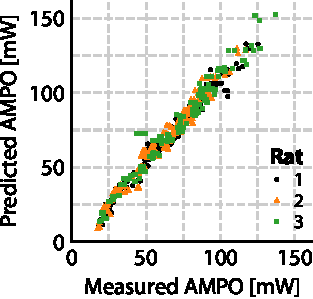
\includegraphics[keepaspectratio]{../figures/r_correlation.pdf}}

}

\caption{\label{fig-r-correlation}\textbf{Comparison of experimentally
measured and predicted AMPO.} Measured AMPO was derived from
experimentally observed MTC length and GM force. Predicted AMPO was
derived using a Hill MTC-type model, with experimentally measured MTC
length and stimulation over time as inputs to predict GM force. Each dot
represents AMPO of one full cycle where muscle stimulation was present,
such that there are three dots for each experimental SSC condition. The
nearly perfect correlation demonstrates that a Hill-type MTC model can
accurately predict the influence of MTC length and stimulation over time
on AMPO.}

\end{figure}%

\paragraph{Imposed stretch--shortening cycles --- constant MTC
shortening/lengthening
velocity}\label{imposed-stretchshortening-cycles-constant-mtc-shorteninglengthening-velocity-1}

Using the Hill-type MTC model, we predicated that AMPO peaks at a value
of 169 mW (averaged across the three rats) at cycle frequency of 3.5 Hz,
an FTS of 0.85 and an MTC length excursion of 8 mm
(Fig~\ref{fig-r-contour} \& Fig~\ref{fig-r-interrelationships}). The
optimal FTS remained remarkably constant across all tested combinations
of cycle frequency and MTC length excursion
(Fig~\ref{fig-r-interrelationships}). By contrast, cycle frequency and
MTC length excursion showed a strong interaction, such that when cycle
frequency was increased, the optimal MTC length excursion decreased, and
vice versa (Fig~\ref{fig-r-interrelationships}). Notably, a broad range
of combinations of SSC parameters achieved AMPO values close to its peak
value (Fig~\ref{fig-r-contour} and Fig~\ref{fig-r-interrelationships}).
For instance, cycle frequency ranging between 2.9 and 4.6 Hz produced an
AMPO within 95\% of maximum AMPO, when adjusting FTS and MTC length
excursion accordingly. For FTS this was a range between 0.74 and 0.91,
when adjusting cycle frequency and MTC length excursion accordingly,
while it was between 6.2 and 10.3 mm for the MTC length excursion when
adjusting cycle frequency and FTS accordingly. These findings
demonstrate that while a clear optimum exists for maximal AMPO, there is
a wide variety of combinations of SSC parameters that yield near-maximal
AMPO values.

\begin{figure}[H]

\centering{

\pandocbounded{
\includegraphics[keepaspectratio]{../figures/r_contour.pdf}}

}

\caption{\label{fig-r-contour}\textbf{Predicted maximally attainable
AMPO as a function of cycle frequency and MTC length excursion, shown
for four distinct FTS values.} The maximally attainable AMPO (in mW),
averaged across three rats, is depicted as contour lines. The open
triangles indicate the location of peak AMPO at each FTS corresponding
to the optimal combination of cycle frequency and MTC length excursion
for each FTS, with the corresponding peak AMPO labelled at the top-left
of the triangle.}

\end{figure}%

\newpage

\begin{figure}[H]

\centering{

\pandocbounded{
\includegraphics[keepaspectratio]{../figures/r_interrelationships.pdf}}

}

\caption{\label{fig-r-interrelationships}\textbf{Predicted
interrelationships between cycle frequency (CF), FTS, MTC length
excursion (\(\Delta L_{MTC}\)) and the maximally attainable AMPO.} These
plots collectively illustrate how cycle frequency, FTS, and MTC length
excursion interact to maximise AMPO under different conditions. This
figure presents a 3x3 grid of plots created by imposing one SSC
parameter at a time while optimising the two other SSC parameters to
maximise AMPO. In the first column, cycle frequency was imposed, and
AMPO (A1) was maximised by identifying the optimal FTS (A2) and MTC
length excursion (A3) at each cycle frequency. In the second column, FTS
was imposed, and AMPO (A1) was maximised by identifying the optimal MTC
length excursion (B2) and cycle frequency (B3) at FTS. In the third
column, MTC length excursion was imposed, and AMPO (C1) was maximised by
identifying the optimal cycle frequency (C2) and FTS (C3) at each MTC
length excursion. For all columns, muscle stimulation onset time and
duration were optimised to maximise AMPO.}

\end{figure}%

\paragraph{Imposed stretch--shortening cycles --- optimal MTC
shortening/lengthening
velocity}\label{imposed-stretchshortening-cycles-optimal-mtc-shorteninglengthening-velocity-1}

Using the Hill-type MTC model, we identified the optimal CE length over
time for maximal AMPO without imposing any constraints on MTC length
over time. We found that AMPO was maximised when CE shortened at an
approximately constant velocity during the shortening phase and
lengthened with increasing velocity during the lengthening phase (see
Fig~\ref{fig-r-oc}), across all imposed cycle frequencies. Given CE
length and CE force over time (and PEE and SEE properties), the
corresponding MTC length over time can be calculated. Thus, MTC length
over time is inherently dependent on the properties of SEE. Because SEE
force is not constant during CE shortening, the MTC velocity that
maximises AMPO is generally not constant during the shortening phase;
even if CE shortening velocity is constant. The size of this effect
depends on the SEE slack length: with a typical slack length
(e.g.~28\,mm), the MTC velocity is clearly not constant (see
Fig~\ref{fig-r-oc}E), whereas with a short slack length (e.g.~3\,mm),
the MTC velocity closely resembles the CE velocity and is therefore
nearly constant during shortening (see Fig~\ref{fig-r-oc}F).

\begin{figure}[H]

\centering{

\pandocbounded{
\includegraphics[keepaspectratio]{../figures/r_oc.pdf}}

}

\caption{\label{fig-r-oc}\textbf{Predicted CE behaviour for maximally
attainable AMPO, shown at three distinct cycle frequencies for rat 1.}
CE length (A), CE force (B), CE velocity (C) and instantaneous
mechanical power output (IMPO) (D) as a function of normalised time
(i.e.~time divided by the cycle duration). CE stimulation was maximal
during the period indicated by the coloured bars and fully off
elsewhere. The right labels depict the normalised values, where CE
length and CE velocity are normalised to optimum CE length, CE force is
normalised to maximal isometric CE force and IMPO is normalised to the
product of optimum CE length and maximal isometric CE force. Based on CE
length and force over time, and the SEE properties, the MTC length over
time can be calculated. The resulting MTC length over time substantially
differs between a typical SEE slack length of 28\,mm (E) and a short SEE
slack length of 3\,mm (F).}

\end{figure}%

For a short SEE slack length, the MTC length over time that maximises
AMPO has a near-constant shortening and lengthening velocity. As a
result, the maximally attainable AMPO using the optimised CE length over
time was only 2 ± 1\% higher than that achieved with constant MTC
shortening and lengthening velocities with a short SEE slack length. It
should be noted, however, that this small increase in AMPO is specific
to imposing cycle frequency. When imposing FTS or MTC length excursion,
the optimal CE length over time was substantially different from that
with constant MTC velocities during shortening and lengthening --
especially at suboptimal values. For the interested reader, we refer to
the Supporting information ({\nameref{S3_File}}) for the effect of FTS
or MTC length excursion on the optimal MTC behaviour for maximising
AMPO.

\subsection{Discussion}\label{discussion}

The aim of this study was to explore the influence of SSC parameters ---
cycle frequency, FTS and MTC length excursion --- on the maximally
attainable AMPO of rat GM. To this end, we combined \emph{in situ}
experiments with simulations and optimisations using a Hill-type MTC
model. Model parameter values were estimated individually for each
specimen based on independent data from quick-release, step-ramp and
isometric experiments. Additionally, the model inputs (i.e.~MTC length
and stimulation over time) were directly derived from the experimental
SSC data. The correlation coefficients between model-predicted and
measured AMPO were nearly perfect (r\textsuperscript{2} \textgreater{}
0.98). This is a remarkable result, particularly given that the
predictions were not tuned to any of the experimental SSCs. This strong
correspondence enabled us to leverage both experimental findings and
model-based predictions to investigate how SSC parameters influence the
maximally attainable AMPO.

Both experimental data and model-based predictions showed that the MTC
should spend substantially more time shortening than lengthening in
order to maximise AMPO --- at an FTS of approximately 0.85. This optimal
FTS value remained remarkably constant across all tested combinations of
cycle frequency and MTC length excursion. By contrast, cycle frequency
and MTC length excursion showed a strong interaction, such that when
cycle frequency increased, the optimal MTC length excursion decreased,
and vice versa. Lastly, we found that AMPO peaked at a cycle frequency
of 3.5 Hz, an FTS of 0.85 and at an MTC length excursion of 8 mm, with a
relatively constant CE velocity throughout the shortening phase and an
increasing CE lengthening velocity throughout the lengthening phase.

\subsubsection{Robustness and reliability of experimental
results}\label{robustness-and-reliability-of-experimental-results}

In previous studies, it has been well established that cycle frequency
and MTC length excursion significantly affect the maximally attainable
AMPO
\citep[e.g.][]{altringham_modelling_1990, askew_effects_1997, askew_optimal_1998, caiozzo_determinants_1997, james_mechanical_1995, james_isometric_1996},
whereas the effect of FTS has only been demonstrated by Askew \& Marsh
{\citep{askew_effects_1997, askew_optimal_1998}}. Our experimental
results also showed significant effects of cycle frequency and FTS on
the maximally attainable AMPO, confirming the sensitivity of AMPO to SSC
parameters. Understanding how these SSC parameters interact to influence
maximally attainable AMPO requires exploring a larger range of muscle
lengths and stimulation timings than is experimentally feasible.
Therefore, we complemented experiments with simulations and
optimisations using a Hill-type MTC model. For this extensive modelling
approach into the influence of SSC parameters on maximally attainable
AMPO, it was crucial that the model could accurately predict
experimental outcomes. Accordingly, our experimental design focused on
selecting a representative and informative set of SSCs to evaluate
model-based predictions. To assess the reliability of our experimental
outcomes, we repeated experimental conditions with similar stimulation
timing (three cycles) and with two different timings. The experimental
results were highly consistent across the tested specimens. Both the
effects of SSC parameters on maximally attainable AMPO (see
Fig~\ref{fig-r-ampo-cf-fts}) and the estimated muscle properties (see
Table~\ref{tbl-r-musprop}) showed minimal inter-individual variation.
This aligns with previous findings showing highly reproducible
mechanical behaviour in muscles of genetically similar animals, making
it unlikely that adding additional animals would change the study
outcomes. Furthermore, the effects of SSC parameters on maximally
attainable AMPO in our study are in strong agreement with prior findings
(see sections below). Taken together, we conclude that our experimental
data are robust and provide a reliable basis to evaluate model
predictions.

\subsubsection{Optimal FTS for AMPO was relatively constant across all
SSC
conditions}\label{optimal-fts-for-ampo-was-relatively-constant-across-all-ssc-conditions}

Our results show that the maximally attainable AMPO substantially
increased when FTS increased from 0.25 to 0.50, regardless of cycle
frequency and/or MTC length excursion. For example, at the optimal
combination of cycle frequency and MTC length excursion, increasing FTS
from 0.25 to 0.50 caused AMPO to increase by about 95\%. This finding is
consistent with the results of {Askew \& Marsh
\citep{askew_effects_1997}}, who reported increases of
\textasciitilde90\% for \emph{m. soleus} and \textasciitilde70\% for
\emph{m. extensor digitorum longus} when FTS increased from 0.25 to
0.50. Further increasing FTS from 0.50 to 0.75 yielded an additional
30\% increase in AMPO, aligning with Askew \& Marsh's observations of a
\textasciitilde40\% increase in AMPO for both muscles. Moreover, {Askew
\& Marsh \citep{askew_effects_1997}} observed that AMPO increased even
further, and peaked at an FTS between 0.80 and 0.90 at the optimal
combination of cycle frequency and MTC length excursion. Our results not
only corroborate this finding, but also demonstrate that the optimal FTS
was relatively constant (ranging 0.84--0.88) across all tested cycle
frequencies (0.5--6 Hz) and MTC length excursions (2--11 mm).

The optimal FTS reflects mainly a trade-off between the CE concentric
force--velocity relationship and excitation dynamics. The negative
effects of both the CE force--velocity relationship and excitation
dynamics on net mechanical work per cycle increase with cycle frequency.
Yet, the fact that the optimal FTS remains relatively constant across
all cycle frequencies studied suggests that these negative effects
increase to a similar extent with cycle frequency
(Fig~\ref{fig-r-interrelationships}). Moreover, because the negative
effects of the CE force--velocity relationship and excitation dynamics
on AMPO are both strongly and comparably linked to muscle fibre type
\citep{close_dynamic_1972}, their combined influence is likely
relatively similar across muscles with different fibre type
compositions. Consequently, it is perhaps not surprising that the
optimal FTS for AMPO remains relatively consistent across different
muscles (\textasciitilde0.85 for rat \emph{m. gastrocnemius medialis} in
this study; \textasciitilde0.85 for mouse \emph{m. soleus} and \emph{m.
extensor digitorum longus} \citep[see][]{askew_effects_1997} and
\textasciitilde0.80 for human \emph{m. quadriceps femoris}
\citep[see][]{reuvers_what_2026}). Together, these findings suggest that
the optimal FTS is not only relatively constant across all SSC
conditions, but also across different species and muscles (with varying
fibre types).

\subsubsection{Effect of FTS on optimal cycle frequency and MTC length
excursion for maximising
AMPO}\label{effect-of-fts-on-optimal-cycle-frequency-and-mtc-length-excursion-for-maximising-ampo}

While the optimal FTS remained relatively constant across all cycle
frequencies and MTC length excursions, FTS itself strongly influenced
the optimal values of both cycle frequency and MTC length excursion
(Fig~\ref{fig-r-interrelationships}). With respect to cycle frequency,
we observed that the optimal value increased with FTS, although the
magnitude of this increase diminished at higher FTS values. This
observation aligns well with findings by {Askew \& Marsh
\citep{askew_effects_1997}}, who reported comparable increases across
FTS values for both \emph{m. soleus} and \emph{m. extensor digitorum
longus}. For MTC length excursion, we found that the optimal value
increased with 25\% and 10\% when raising FTS from 0.25 to 0.50 and from
0.50 to 0.75, respectively. A direct comparison with {Askew \& Marsh
\citep{askew_effects_1997}} is difficult, as their results differed
between muscles: for \emph{m. soleus}, these increases were 35\% and
40\%, while they were 0\% and 35\% for \emph{m. extensor digitorum
longus}. Lastly, {Askew \& Marsh \citep{askew_effects_1997}} also
examined how average muscle shortening velocity varied with FTS. For
\emph{m. extensor digitorum longus}, they found a consistent decrease in
optimal shortening velocity as FTS increased. By contrast, \emph{m.
soleus} showed a slight increase in optimal shortening velocity,
although this discrepancy may stem from missing data near the optimal
frequency at FTS = 0.75 (see their Figure 4). A follow-up study by the
same authors \citep{askew_optimal_1998} later confirmed that the optimal
average shortening velocity for \emph{m. soleus} indeed decreases with
increasing FTS, independently of cycle frequency. We observed the same
for our model-predictions. Overall, our findings regarding the influence
of FTS on optimal cycle frequency, MTC length excursion, and average
shortening velocity are in line with previous literature. These findings
are not surprising, given the effect of the CE force--velocity
relationship. After all, at higher FTS, there is relatively more time
for shortening than at lower FTS values. This enables an increase in
cycle frequency and allows muscles to shorten and lengthen over a
greater distance, without substantial negative effects due to the effect
of shortening velocity on muscle force.

\subsubsection{Optimal cycle frequency and optimal MTC length excursion
for maximal
AMPO}\label{optimal-cycle-frequency-and-optimal-mtc-length-excursion-for-maximal-ampo}

While the optimal FTS for maximal AMPO remained relatively constant
across all SSCs studied, we found that cycle frequency and MTC length
excursion strongly interacted for maximal AMPO. Specifically, as cycle
frequency increased, the optimal MTC length excursion for the maximally
attainable AMPO decreased, and vice versa (see Fig~\ref{fig-r-contour}
\& Fig~\ref{fig-r-interrelationships}). This interaction has previously
been observed in sinusoidal SSCs \citep[e.g.][]{james_isometric_1996} --
where shortening and lengthening durations are equal. A similar
interaction between cycle frequency (i.e.~cadence) and crank
length---which influences MTC length excursion---has also been observed
in human sprint cycling \citep[e.g.][]{martin_determinants_2001}, where
shortening and lengthening durations of individual MTCs are not
necessarily equal. However, to our knowledge, this interaction has not
been systematically examined in controlled SSCs with systematically
varied unequal shortening and lengthening durations; although {Askew \&
Marsh \citep{askew_effects_1997}} briefly noted this interaction, they
did not present the relevant data.

The interaction between cycle frequency and MTC length excursion for
maximally attainable AMPO did not come as a surprise, given the negative
effect of the CE force--velocity relationship on AMPO. In line with
{Askew \& Marsh \citep{askew_effects_1997}}, {Caiozzo \& Baldwin
\citep{caiozzo_determinants_1997}} and {James et al.
\citep{james_isometric_1996}}, we observed that the maximally attainable
AMPO was less sensitive to increases in cycle frequency and MTC length
excursion above their respective optimal values than to decreases below
these optimal values. This is not only true at optimal FTS (see
Fig~\ref{fig-r-interrelationships}), but also at suboptimal FTS. The
latter can be observed in Fig~\ref{fig-r-contour}, where the contour
lines are more closely spaced below than above the optimum cycle
frequency and MTC length excursion. This indicates that, for a given
change in cycle frequency or MTC length excursion, AMPO decreases more
rapidly below the optimal value than above it. The finding that AMPO was
less sensitive to increases in cycle frequency and MTC length excursion
above their respective optimal values than to decreases below these
optimal values might be counter-intuitive, as one may expect the
maximally attainable AMPO to decline rapidly due to a higher shortening
velocity (at higher cycle frequencies and MTC length excursion).
However, at low cycle frequencies, the MTC must shorten and lengthen
over a substantial distance, which reduces the maximally attainable AMPO
primarily due the effect of the CE force--length relationship.
Conversely, at low MTC length excursions, very high cycle frequencies
are required to achieve substantial power output, which in turn
compromises AMPO due to the effect of the CE force--velocity
relationship (i.e.~muscle contracts at lengths at which CE force is
substantially lower than the maximal isometric force). In sum, our
findings indicate that deviations above the optimal cycle frequency and
MTC length excursion have a less detrimental effect on the maximally
attainable AMPO than deviations below optimal values.

\subsubsection{Effect of SEE properties on the MTC behaviour for maximal
AMPO}\label{effect-of-see-properties-on-the-mtc-behaviour-for-maximal-ampo}

To maximise AMPO, CE should shorten at an approximately constant
velocity during the shortening phase and lengthen with increasing
velocity during the lengthening phase (see Fig~\ref{fig-r-oc}). The
resulting MTC length over time for maximal AMPO is determined not only
by CE length over time, but also by the SEE properties (i.e.~SEE
compliance and SEE slack length). Due to SEE elasticity, MTC velocity
should be higher (i.e.~less negative or even positive) than that of CE
during force development, and lower (i.e.~more negative) during force
relaxation to maximise AMPO (Fig~\ref{fig-r-oc}E).

The same principle applies the other way around: when velocity of MTC is
constant, that of CE varies during force development and relaxation.
Specifically, changes in CE velocity increase with increasing SEE
compliance and SEE slack length. In the experimentally observed SSCs,
the estimated SEE slack length was substantially longer
(\textasciitilde28 mm) than that used in the simulated SSCs (3 mm),
resulting in more variable CE velocity during shortening. This variable
CE velocity compromises AMPO: for a given shortening distance, CE should
ideally shorten at a constant velocity to maximise AMPO. This more
variable CE velocity during the shortening phase of the experimental SSC
was the main reason why AMPO in the experimental SSCs was lower than in
the simulated SSCs. For instance, at a 2 Hz cycle frequency, FTS of 0.5
and an 8 mm MTC length excursion, AMPO in the simulated SSC was
\textasciitilde40\% higher (\textasciitilde80 mW vs.~\textasciitilde110
mW; Fig~\ref{fig-r-ampo-cf-fts} vs. Fig~\ref{fig-r-contour}).

We found that -- especially at a low FTS, a high cycle frequency and a
small MTC length excursions -- muscle stimulation should occur before
MTC shortening starts in order to maximise AMPO. Consequently, CE
shortening started before MTC shortening, such that CE was shortening
over a longer time interval resulting in a lower average CE shortening
velocity than MTC. Thus, the behaviour of SEE does not only cause a
discrepancy between instantaneous CE and MTC velocity, it also affects
their average shortening velocities.

{Askew \& Marsh \citep{askew_optimal_1998}} reported that at low FTS
values and high cycle frequencies, the average MTC shortening velocity
exceeded the CE velocity that maximises instantaneous power output based
on the force--velocity relationship (\(v_{CE}^{opt}\)). They
acknowledged that this was a unexpected finding, since CE shortening
velocity should theoretically be at or below \(v_{CE}^{opt}\) in order
to maximise AMPO. Similar to our SSCs with a constant MTC shortening and
lengthening velocity, {Askew \& Marsh \citep{askew_optimal_1998}} left a
small portion of the tendon attached to the muscle fibres. Since Askew
\& Marsh reported that muscle stimulation onset occurred before MTC
shortening it is evident that average CE shortening velocity was lower
than that of MTC. Therefore, their finding that optimal CE shortening
velocity should exceeds \(v_{CE}^{opt}\) can, at least, partly be
attributed to an overestimation of CE shortening velocity due to the
series elastic structures.

The discrepancy between CE and MTC shortening velocity is most
pronounced at low FTS, high cycle frequencies, and small MTC length
excursion --- exactly where {Askew \& Marsh \citep{askew_optimal_1998}}
observed CE shortening velocities exceeding \(v_{CE}^{opt}\). At high
FTS values, however, this discrepancy is lower. {Askew \& Marsh
\citep{askew_optimal_1998}} found that at high FTS values (i.e.~0.75),
the optimal average shortening velocity was consistently below
\(v_{CE}^{opt}\). This aligns with our findings, even when muscle
stimulation onset preceded MTC shortening. In conclusion, while other
factors may play a role, we are confident that such factors have little
influence on the effect of SSC parameters on the maximally attainable
AMPO near the optimum.

\subsubsection{Applications of findings}\label{applications-of-findings}

In most real-world situations, SSCs of individual muscles emerge from
the interaction between the musculoskeletal system and the environment.
Consequently, the extent to which SSC parameters can be influenced
depends on the mechanical context of the task. During flying, for
example, birds can and do actively adjust wing kinematics (e.g.~by
folding and unfolding their wings), thereby enabling a longer shortening
than lengthening duration of \emph{m. pectoralis major}
\citep[e.g.,][]{askew_mechanical_2001, biewener_vivo_1998, earls_kinematics_2000, ellerby_modulation_2007, jackson_scaling_2011, spedding_wake_1987, williamson_pectoralis_2001}.
Our findings help to understand this, as a longer shortening duration is
favourable for maximising AMPO. In addition, our results may also shed
light on (the evolution of) the ``design'' of musculoskeletal systems,
for example the role of moment-arms which affect MTC length excursion
thereby influencing AMPO \citep[e.g.][]{polet_optimal_2024}

SSC parameters can be substantially influenced by modifying the
interaction between the musculoskeletal system and the environment. One
way to achieve this is through the use of external equipment, which can
change or constrain movement kinematics. A prime example of such
equipment is the bicycle, where crank length affects joint excursions
and thus MTC length excursions. Also, non-circular chainrings can be
used to vary the gear ratio throughout the crank revolution. This allows
the gear ratio to be increased during the downstroke and to be decreased
during the upstroke, thereby changing the relative time spent in each
phase. In a clever experiment, {Martin et al. \citep{martin_pedal_2002}}
manipulated chainring shape to alter the relative duration of the
downstroke and upstroke during single-leg sprint cycling. AMPO increased
with a greater proportion of time spent in the downstroke: an 18\%
increase was observed when the downstroke occupied 50\% rather than 42\%
of the cycle duration, and a further 4\% increase was observed at 58\%
compared to 50\%. Another example is rowing, where the resistance during
the stroke and recovery phases could be adjusted in order to alter
muscle shortening and lengthening durations. More broadly, such
(re)design principles could be applied to any equipment that changes or
constrains movement kinematics, thereby enabling the SSCs of the
involved muscles to operate closer to their optimum for AMPO.

It should be noted that in motor activities involving multiple muscles
(e.g., bicycling, handcycling, rowing, speed skating, etc.), the
objective is not to maximise the AMPO of a single muscle. Rather, the
goal is to maximise the total AMPO of all muscles combined, which
introduces an additional trade-off. In this context, when considering a
joint, it should be clear that the optimum FTS for one muscle (e.g.~an
FTS of \textasciitilde0.85) cannot be realised in both agonists and
antagonists. In this situation, the optimal solution arises from a
trade-off that depends on properties of both muscles (e.g.~maximal
isometric force and muscle fibre length), and is therefore expected to
shift in both muscles towards more intermediate values (i.e.~closer to
an FTS of 0.5). Nevertheless, it stands to reason that larger muscles
should operate closer to their individual optimum than smaller muscles
in order to maximise performance. Thus, when (re-)designing equipment to
maximise total AMPO, configurations should enable larger muscles to
operate closer to their individual optimum. Our study provides a
starting point for guiding future equipment design aimed at improving
total AMPO.

\newpage{}

\phantomsection

\subsection*{Supporting information}\label{supporting-information}
\addcontentsline{toc}{subsection}{Supporting information}

\paragraph{S1 Table.}\label{s1-table.}

\label{S1_Table} \textbf{Overview of experimental stretch--shortening
cycle conditions with a 4 mm MTC length excursion.} The table summarises
the SSC parameters, stimulation duration, and measured AMPO for each
rat.

\paragraph{S2 Table.}\label{s2-table.}

\label{S2_Table} \textbf{Overview of experimental stretch--shortening
cycle conditions with an 8 mm MTC length excursion.} The table
summarises the SSC parameters, stimulation duration, and measured AMPO
for each rat.

\paragraph{S1 File.}\label{s1-file.}

\label{S1_File} \textbf{Selection of experimental SSC conditions.}
Description of the preliminary Hill-type muscle--tendon complex
simulations used to determine the experimental stretch--shortening cycle
(SSC) conditions.

\paragraph{S2 File.}\label{s2-file.}

\label{S2_File} \textbf{Optimisation protocol to identify optimal MTC
length over time.} Description of the optimal control problem to find
the fully unconstrained MTC length and stimulation over time that
maximises AMPO.

\paragraph{S3 File.}\label{s3-file.}

\label{S3_File} \textbf{Optimal CE length over time: influence of FTS
and MTC length excursion.} Detailed results of the predicted optimal MTC
length over time for maximising AMPO under imposed FTS values and MTC
length excursions.

\phantomsection

\subsection*{Acknowledgments}\label{acknowledgments}
\addcontentsline{toc}{subsection}{Acknowledgments}

The authors thank Guus Baan for creating the illustration used in Figure
3.

\phantomsection

\subsection*{Competing interests}\label{competing-interests}
\addcontentsline{toc}{subsection}{Competing interests}

The authors declare no competing or financial interests.

\phantomsection

\subsection*{Author contributions}\label{author-contributions}
\addcontentsline{toc}{subsection}{Author contributions}

Conceptualization: E.D.H.M.R., D.A.K.; Formal analysis: E.D.H.M.R.;
Funding acquisition: D.A.K.; Investigation: E.D.H.M.R., W.N.;
Methodology: E.D.H.M.R., H.M., D.A.K.; Resources: H.M., Software:
E.D.H.M.R.; Supervision: H.M., M.F.B., D.A.K.; Visualization:
E.D.H.M.R.; Writing - Original Draft: E.D.H.M.R.; Writing - Review \&
Editing: E.D.H.M.R., H.M., M.F.B., D.A.K.;

\phantomsection

\subsection*{Funding}\label{funding}
\addcontentsline{toc}{subsection}{Funding}

This work was funded by The Dutch Research Council (NWO)~{[}21728 to
D.A.K.{]}.

\phantomsection

\subsection*{Data and resource
availability}\label{data-and-resource-availability}
\addcontentsline{toc}{subsection}{Data and resource availability}

All data, code, and materials used in this study are openly available:

\begin{itemize}
\item
  \textbf{GitHub repository:} All raw data, processed data, and analysis
  code are hosted on GitHub at
  \url{https://github.com/edwinreuvers/rat-gm-ampo}.
\item
  \textbf{Reproducible analysis website:} Full analysis pipeline ---
  including data, analysis code, and figure/table generation --- is
  available at
  \url{https://edwinreuvers.github.io/publications/rat-gm-ampo}.
\end{itemize}

\newpage{}

\phantomsection

\subsection*{References}\label{references}
\addcontentsline{toc}{subsection}{References}

\renewcommand{\bibsection}{}
\bibliography{../_resources/references.bib}

\newpage{}


\nolinenumbers


\end{document}
